\chapter{Implementation}
\label{chap:impl}
This chapter analyzes specifics of Odin (short for Object Dependency INspector) - a static analyzer of EO source code. Section 4.1 covers the tools and technologies used in the project. Section 4.2 gives a brief overview of the project file structure.
Section 4.3 goes over the implementation of EO parser used in the project. Section 4.4 discusses the ways we can represent the elements of object-oriented programs in EO. Sections 4.5 and 4.6 describe the implementations of the analysis algorithms applied to structured EO code. Finally, section 4.7 summarizes this chapter.

\section{Development Environment}
Odin is a project written entirely in \textbf{Scala} \footnote{\url{https://www.scala-lang.org/}} - a modern programming language with support for high-level concepts such as structural pattern matching \cite{pattern_matching} and algebraic data types \cite{adts}. Scala is compiled into Java Virtual Machine (JVM) byte code. This allows Odin to be used as a library in any other project compatible with JVM, be it Scala or Java. In addition, programs compiled to JVM byte code can be run without changes on any device that can run Java Virtual Machine.


The project uses a build tool called \textbf{sbt} \footnote{\url{https://www.scala-sbt.org/}}, which allows compiling multiple Scala modules at once. A distinctive feature of \textbf{sbt} is the ability to cross-compile Scala code so that it is compatible with many versions of Scala and Java. It also supports a variety of plugins that improve the development process. The plugins used by Odin are \textbf{scalafmt} \footnote{\url{https://scalameta.org/scalafmt/}}, an automatic source code formatter, and \textbf{scalafix} \footnote{\url{https://scalacenter.github.io/scalafix/}} , a linter and code analyzer with support for project-wide refactorings.

Odin is published as a \textbf{JAR} \footnote{\url{https://docs.oracle.com/javase/7/docs/technotes/guides/jar/jar.html}} and can be downloaded from the \textbf{Maven Central} repository \footnote{\url{https://search.maven.org/search?q=g:org.polystat.odin}}.

The source code of the project is available on \textbf{Github} \footnote{\url{https://github.com/polystat/odin}}. It also provides the instructions on how to launch and contribute to the project.



\section{Module Structure}
Odin is a project consisting of multiple modules. The main modules are:
\begin{itemize}
    \item Core, which contains the definition for EO AST (Abstract Syntax Tree).
          This AST is used as an input to all analysis algorithms.
    \item Analyses, which contains the implementations of various analyzers.
    \item Backends, which contains algorithms that transform EO AST into something else. The only backend so far is a plain text backend: it transforms EO AST into its syntactically correct equivalent in EO source code. This backend can also be interpreted as a pretty-printer of EO code and is widely used as such in other modules.
    \item Parser, which contains a parser (also known as a syntactic analyzer) of EO source code. It is used to convert different EO representations (e.g. plain text or XML encoding) into the EO AST defined in Core module.
\end{itemize}
\section{Parser}
The parser used in Odin implements a slightly altered version of EO specification defined by Bugayenko \cite{eolang}. In particular, it relaxes constraints on whitespace between tokens and the number of newlines and comments between definitions. This is done to reduce the complexity of producing source code pieces for testing and debugging.


The parser was created using \textbf{cats-parse} library \footnote{\url{https://github.com/typelevel/cats-parse}} for Scala. It provides a parser-combinator \cite{hill_combinators_1996} approach to building recursive-descent parsers. Recursive-descent parsers are known for their worst-case exponential complexity. This problem can not be avoided in general. However, cats-parse mitigates it by explicitly marking all the places in the parser definition that can cause such spikes in complexity.

\section{Analyses}
This section describes each of the analysis algorithms in greater detail. First, we will describe the steps that are performed prior to each of the defect-specific analyses: parsing and detecting the significant features of EO programs - objects, methods and extension clauses. Then we will describe the algorithms for detecting each of the covered defects: unanticipated mutual recursion and unjustified assumption in subclass. Finally, we will conclude the chapter by describing the shortcomings of each of the algorithms.


\subsection{Preprocessing}
Before running on


\section{Detecting Unanticipated Mutual Recursion}
\label{impl:mutualrec}

\subsection{Proposed solution}
The solution to the problem lies in detecting the cycles in the call-graphs of all the objects. For each class-object in the program, do the following:
\begin{enumerate}
    \item Detect the decorated class-object, all methods, and for each method in the class detect all the methods it calls. If the method that is called exists in the class-object, mark it as \textit{resolved}. Otherwise, mark it as \textit{partially-resolved}. The set of mappings between the methods of the class and the methods that each of the methods calls is considered a \textit{partial call-graph} of the object.
    \item After that the tree is traversed again to convert all the partially-resolved calls to fully resolved calls. To do that we need to calculate the \textit{complete call-graph} of the object, which contains the methods from the object itself, as well as the methods from the decorated object. This is done by \textit{extending} the partial call-graph of the decorated object with the partial call-graph of the decorating objects. Hereinafter we use the terms \textbf{child} and \textbf{parent} to refer to the decorating object and the decorated object respectively. The extension procedure is defined as follows: 
    \begin{enumerate}
        \item if the method is present in the parent call-graph, but is absent in the child call-graph, it is left as is. 
        \item if the method is present in the child call-graph but does not exist in the parent call-graph, it is added to the parent call-graph.
        \item if the method is present both in the child call-graph and the parent call-graph, all the occurrences of the method in the parent call-graph are replaced by the child's version of the method.
    \end{enumerate} 
    \item After the object's call-graph is resolved, perform the depth-first search \cite{dfs} to find the cycles in the complete call-graph. After all the cycles are found, exclude the cycles that contain only the methods from the same object. 
\end{enumerate}

\section{Detecting Unjustified Assumption in Subclass}
\label{impl:unjustified}

\subsection{Proposed Solution}
We propose the following approach for detecting the methods where inlining of the calls may lead to breaking changes in subclasses:
\begin{enumerate}
    \item An \textit{initial} representation of the program is produced. This representation is a tree-like data structure which preserves the nesting relations between objects. So, the objects which contain other objects are the roots of their respective subtrees, whereas the container objects are the subtrees or leaves.
    \item We produce a \textit{revision} of the initial program representation where all the calls to the methods are inlined. 
    \item In both versions, for each of the class-objects, for each method in the class-object, a set of \textit{properties} is inferred.  These properties can be thought of as an implicit contract \cite{meyer} of each method. In addition to the implicit properties, the explicit properties which come in the form of \textit{assert} statements in the source code are also taken into account. In order to infer the properties of the method, partial interpretation of its body is performed. The interpretation is limited to basic numeric operations, numeric and boolean values and method calls. The inference rules are described in greater detail in fig. \ref{fig:props}.
    \item After all the properties are inferred, the following predicate should hold true for both the initial and the revised versions:
    \begin{align*}
        P_{init} \implies P_{rev}
    \end{align*}
    If it doesn't hold for some class-object, it means that the revision of one of its superclasses introduces a breaking change, which weakens the precondition of some its methods. 
\end{enumerate}

\begin{figure}
    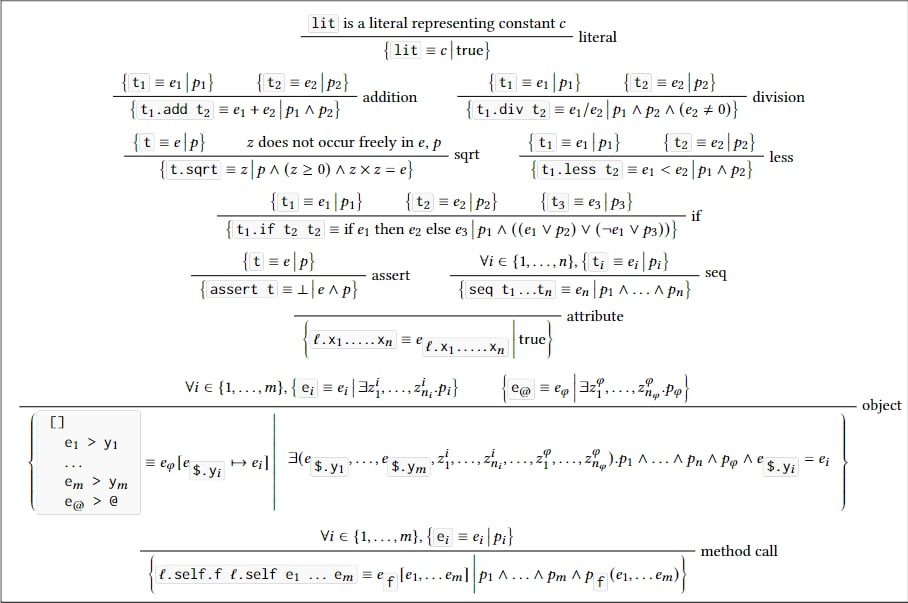
\includegraphics[width=\textwidth]{figs/properties}
    \caption{Rules for property inference in detection of unjustified assumption in subclass.}
    \label{fig:props}
\end{figure}

